\chapter{Architecture and Design}

\epigraph{In general, when modeling phenomena in science and
  engineering, we begin with simplified, incomplete models. As we
  examine things in greater detail, these simple models become
  inadequate and must be replaced by more refined
  models.}{\textit{Structure and Interpretation of Computer Programs,
    Section 1.1.5}\cite{sicp}}

\section{Structure of combox}

combox consists of two main components -- the combox directory and the
node directories. The combox directory is the place where the user
stores all of their files; the node directories are the directories
under which encrypted shards of the files (in the combox directory)
are scattered to. A node directory is the file storage provider's
directory. For instance, the Dropbox directory and the Google Drive
directory are node directories.

When a file, \verb+humans.txt+, is created in the combox directory,
combox splits \verb+humans.txt+ into \verb+N+ shards, where \verb+N+
is the number of node directories. If there are two node directories
(Dropbox directory and Google Drive directory), then 2 shards are
created. Each shard of the file is then encrypted and the encrypted
shards are spread evenly across the node directories. Now, the Dropbox
client and the Google client will sync the respective shards that was
place under their directories to their respective data store.

\begin{figure}[h]
  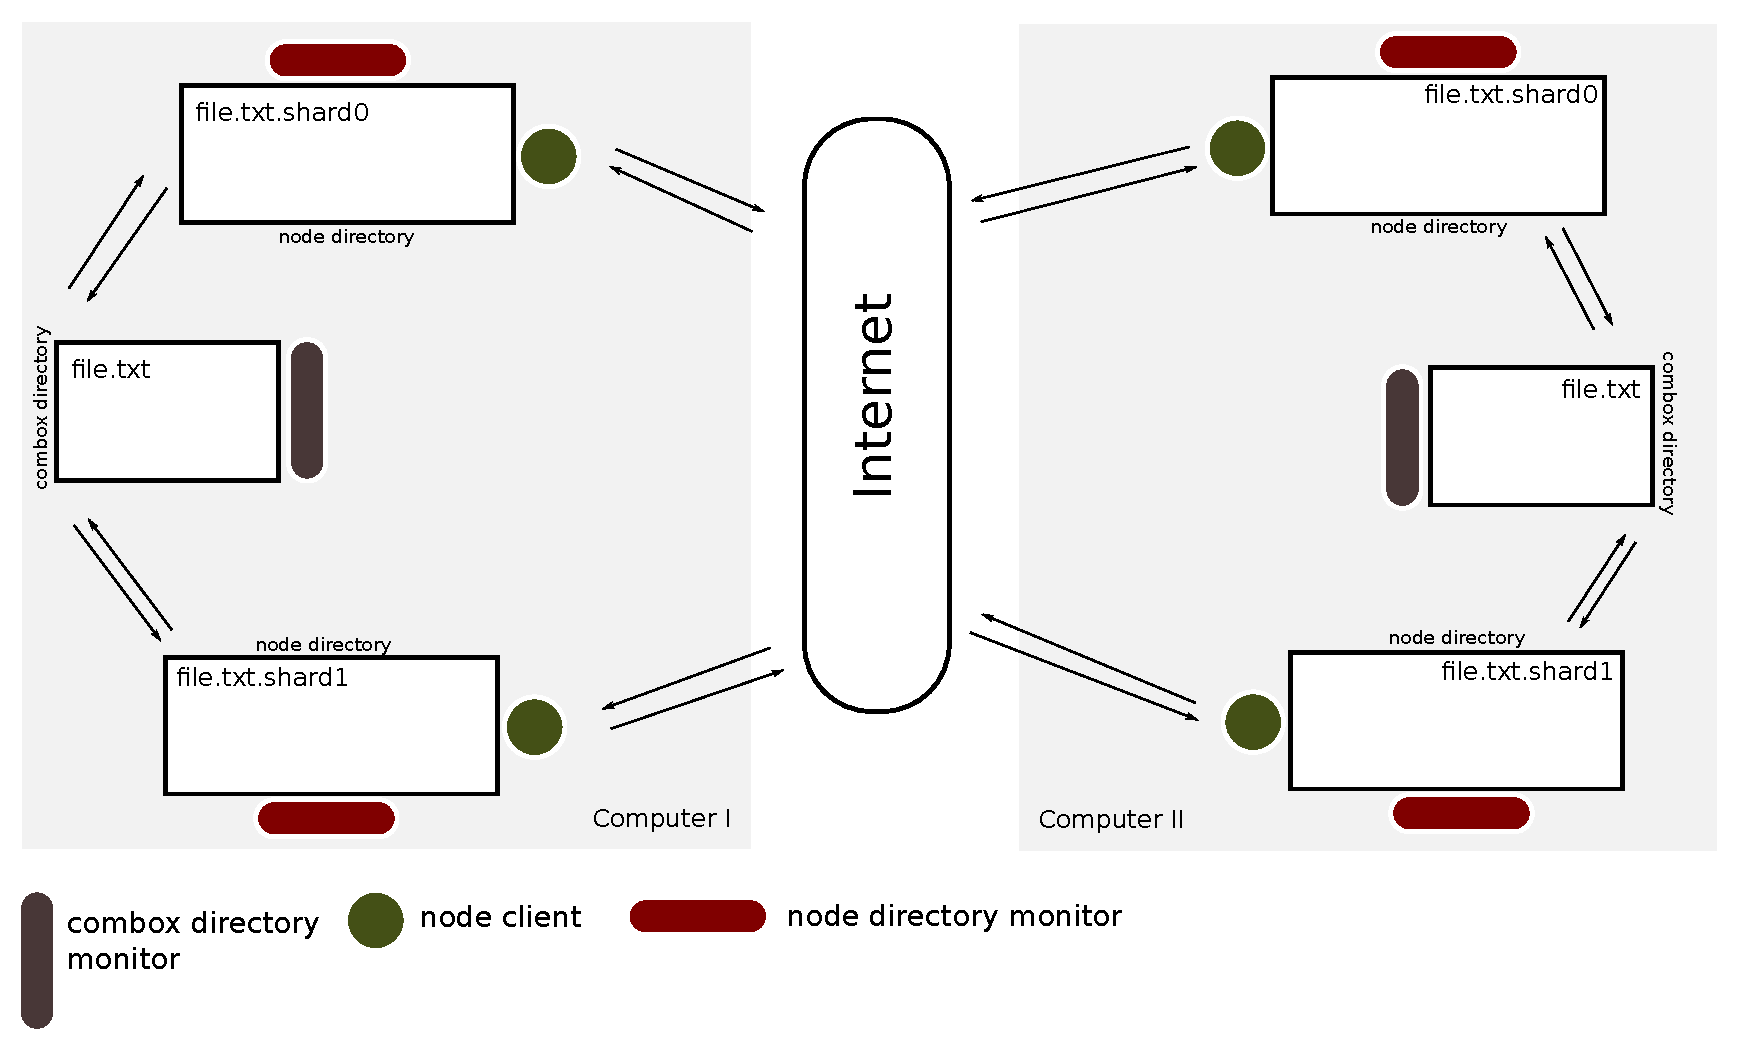
\includegraphics[scale=0.6]{3-combox-structure}
  \caption{High level overview of how file creation works when combox
    is setup on two computers.}
  \label{fig:3-combox-structure}
\end{figure}

Now, when the user moves to their second computer, the node clients
(Dropbox client and the Google Drive client) will sync the new
encrypted shards to their respective directories. Once the encrypted
shards are synced to the node directories, combox will pick the
encrypted shards -- \verb+humans.txt.shard0+, \verb+humans.txt.shard1+
-- decrypt them and reconstruct into \verb+humans.txt+ and place it in
the respective location under the combox directory; figure
\ref{fig:3-combox-structure} illustrates this. The process is similar
for file modification, deletion and rename/move.

\subsection{combox configuration}\label{sec:3-combox-config}

The combox configuration wizard triggers automatically when combox
finds that it is not configured. The combox configuration wizard
configures the combox directory; asks the user to point to the
location of the node directories; and reads the key (passphrase) to be
used to encrypt file shards that are spread across the node
directories. The combox configuration is written to
\verb+$HOME/.combox/config.yaml+. This YAML configuration file can be
manually edited by the user.

The
\verb+config_cb+\footnote{https://git.ricketyspace.net/combox/tree/combox/config.py?id=fb7fdd21\#n90}
function in the \verb+combox.config+ module is responsible for
carrying out the combox configuration. Prior to version \verb+0.2.0+,
the combox configuration was purely done through the Command Line
Interface (CLI). From \verb+0.2.0+ on wards, by default, the combox
configuration is done through a graphical interface; it is still
possible to configure combox through the CLI with the \verb+--cli+
switch.

A demo of combox configuration using the graphical interface on
GNU/Linux can be viewed
\url{https://ricketyspace.net/combox/combox-config-gui-glued-gnu.webm}{here}.
T he same demo of combox configuration using the graphical interface
on OS X can be viewed
\url{https://ricketyspace.net/combox/combox-config-gui-glued-osx.webm}{here}.

\subsection{combox directory monitor}\label{sec:3-combox-cdirm}

combox directory monitor is an instance of
\verb+combox.events.ComboxDirMonitor+\footnote{https://git.ricketyspace.net/combox/tree/combox/events.py?id=fb7fdd21\#n42}
monitoring the combox directory for changes. When changes are made to
the combox directory, the combox directory monitor is responsible for
correctly detecting the type of change and doing the right thing at
that instance of time.

When a file is created in the combox directory, the combox directory
monitor will take that file, split it into \verb+N+ (equal to the
number of node directories) shards, encrypt the shards, spread the
encrypted shards to the node directories, and finally store the hash
of the file in the local combox data store.

When a file is modified in the combox directory, the combox directory
monitor will take that modified file, split it into \verb+N+ (equal to
the number of node directories) shards, encrypt the shards, spread the
encrypted shards to the node directories, and finally update the hash
of the file in the local combox data store.

When a file is deleted in the combox directory, the combox directory
monitor will remove the encrypted shards of the file in the node
directories and get rid of the file's hash from the local combox data
store.

When a file is moved/renamed in the combox directory, the combox
directory monitor will move/rename encrypted shards in all the node
directories, remove the file's hash from the local combox data store
and store the hash of file under its new name.

\subsection{Node directory monitor}\label{sec:3-combox-nodirm}

Node directory monitor is an instance of
\verb+combox.events.NodeDirMonitor+\footnote{https://git.ricketyspace.net/combox/tree/combox/events.py?id=fb7fdd21\#n352}
that monitors a node directory. When changes are made to the node
directory, the node directory monitor is responsible for correctly
detecting the type of change and doing the right thing at that
instance of time. Each node directory has a dedicated node directory
monitor. If there are 2 node directories, then combox will instantiate
2 node directory monitors.

When an encrypted shard is created in the node directory due to a file
created on another computer, the node directory first checks if the
respective file' encrypted shard(s) has/have arrived in other node
directory/directories. If all encrypted shards have arrived, then the
node directory takes all the encrypted shards, decrypts them,
reconstructs the file and puts the file in the combox directory on
this computer and stores the hash of the newly created file in the
local combox data store. If all the encrypted shards have not arrived,
then the node directory does not do anything. It must be observed here
that the node directory monitor of the last node directory which gets
the encrypted shard will be the one to perform the file reconstruction
and creation.

When an encrypted shard is modified in the node directory due to a
file modified on another computer, the node directory first checks if
the respective file' modified encrypted shard(s) has/have arrived in
other node directory/directories. If all modified encrypted shards
have arrived, then the node directory takes all the modified encrypted
shards, decrypts them, reconstructs the file and puts the modified
version of the file in the combox directory on this computer and
updates the file's hash in the local combox data store. If all the
modified encrypted shards have not arrived, then the node directory
does not do anything. It must be observed here that the node directory
monitor of the last node directory which gets the modified encrypted
shard will be the one to perform the file reconstruction and will
place the modified file in the combox directory.

When an encrypted shard is deleted in the node directory due to a file
deleted on another computer, the node directory first checks if the
respective file' encrypted shard(s) has/have been deleted in other
node directory/directories. If all encrypted shards have been deleted
from the node directories, then the node directory deletes the file in
the combox directory on this computer and removes its information from
the local combox data store. If all encrypted shards have not been
deleted, then the node directory does not do anything. It must be
observed here that the node directory monitor of the last node
directory in which the encrypted shard is deleted will be the one to
delete the file from the combox directory.

When an encrypted shard is moved/renamed in the node directory due to
a file moved/renamed on another computer, the node directory first
checks if the respective file' moved/renamed encrypted shard(s)
has/have arrived in other node directory/directories. If all
moved/renamed encrypted shards have arrived, then the node directory
takes all the moved/renamed encrypted shards, decrypts them,
reconstructs the moved/renamed file and puts the moved/renamed file in
the combox directory on this computer and stores the hash under the
file' new name in the local combox data store. If the all the
moved/renamed encrypted shards have not arrived, then the node
directory does not do anything. It must be observed here that the node
directory monitor of the last node directory which gets the
moved/renamed encrypted shard will be the one to perform the file
reconstruction and will place the moved/renamed file in the combox
directory.

\subsection{combox data store}\label{sec:3-combox-db}

To ``keep it simple, stupid'', combox tracks bare minimum information
about the files that are stored in the combox directory, depending on
file system events to do the right thing when changes takes place in
the combox directory.

The only information that is stored in the combox data store with
regards to a file in the combox directory is its SHA-512 hash. The
SHA-512 hash of a file is enough information to detect changes in the
file. In the data store, there are also four dictionaries --
\verb+file_moved+, \verb+file_deleted+, \verb+file_created+,
\verb+file_modified+ -- which track the number of shards of a file
that were moved/deleted/created/modified due the respective file being
moved/deleted/created/modified on another computer. These four
dictionaries are primarily used by the \verb+NodeDirMonitor+ to detect
remote file movement/deletion/creation/modification and triggering
file reconstruction from the encrypted shards at the right time.

The data store is a JSON file on the disk, stored by default at \\
\verb+$HOME/.combox/silo.db+. The
\verb+combox.silo.ComboxSilo+\footnote{https://git.ricketyspace.net/combox/tree/combox/silo.py?id=v0.2.2\#n29}
is the sole interface to read from and write to the data store. The
data store is primarily accessed and modified by the combox directory
monitor (\verb+ComboxDirMonitor+) and the node directory monitor
(\verb+NodeDirMonitor+) through a shared \verb+threading. Lock+ that
ensures that only one entity\footnote{An entity can be the combox
  directory monitor or one of the node directory monitors} can
access/modify the database at a time.

Below is an illustration of the structure of the combox data store:

\begin{verbatim}
{
  "/home/rsd/combox/ipsum.txt": "e3206df2bb2b3091103ab9d...",
  "/home/rsd/combox/tk-shot-osx.png": "7fcf1b44c15dd95e0...",
  "/home/rsd/combox/thgttg-21st.png": "0040eedfc3eeab546...",
  "/home/rsd/combox/lorem.txt": "5851dd7a4870ff165facb71...",
  "/home/rsd/combox/the-red-star.jpg": "4b818126d882e552...",
  "file_moved": {},
  "file_deleted": {},
  "file_created": {},
  "file_modified": {},
}
\end{verbatim}

The \verb+combox.silo.ComboxSilo+, which is the sole interface to read
from and write to the database, uses the pickleDB library
\cite{pylib:pickledb}. The pickleDB is a very basic key-value store
which allows one to store information in the JSON format.

It must be noted that the combox data store on each computer is
independent and does not communicate or make transactions with the
combox data store located in other computers.

\section{combox modules overview}

combox is spread into modules that have functions and/or
classes. Currently, combox is considerably a small program consisting
of the following files:

\begin{verbatim}
$ wc -l combox/*.py
  144 combox/cbox.py
  178 combox/config.py
  241 combox/crypto.py
  891 combox/events.py
  541 combox/file.py
  454 combox/gui.py
    0 combox/__init__.py
   71 combox/log.py
  278 combox/silo.py
   29 combox/_version.py
 2827 total
\end{verbatim}

This section gives an overview of each of the combox modules with
extreme brevity.

\begin{description}
\item[combox.cbox]\footnote{https://git.ricketyspace.net/combox/tree/combox/cbox.py?id=fb7fdd21}
  This module contains \verb+run_cb+ function that starts/initiates
  combox; this function creates an instance \verb+threading.Lock+ for
  combox data store access and another instance of
  \verb+threading.Lock+ which is shared by instances of
  \verb+combox.events.ComboxDirMonitor+ and
  \verb+combox.events.NodeDirMonitor+; it initializes an instance
  \verb+combox.events.ComboxDirMonitor+ that monitors the combox
  directory and an instance of \verb+combox.events.NodeDirMonitor+ for
  each node directory. This modules also houses the \verb+main+
  function that parses commandline arguments, starts combox
  configuration if needed or loads the combox configuration file to
  start running combox.
\item[combox.config]\footnote{https://git.ricketyspace.net/combox/tree/combox/config.py?id=fb7fdd21}
  Accommodates two import functions -- \verb+config_cb+ and
  \verb+get_nodedirs+. The \verb+config_cb+ is the combox
  configuration function that allows the user to configure combox;
  this function was designed in a such way that it could be used by
  both the commandline and graphical interfaces for configuring
  combox. The \verb+get_nodedirs+ function returns, as a list, the
  paths of the node directories; this function use used in numerous
  places in other combox modules.
\item[combox.crypto]\footnote{https://git.ricketyspace.net/combox/tree/combox/crypto.py?id=fb7fdd21}
  This has functions for encrypting and decrypting data; encrypting
  and decrypting shards (\verb+encrypt_shards+ and
  \verb+decrypt_shards+); a function for splitting a file into shards,
  encrypting those shards and spreading them across node directories
  (\verb+split_and_encrypt+); a function for decrypting the shards
  from the node directories, reconstructing the file from the
  decrypted shards and putting the file to the combox directory
  (\verb+decrypt_and_glue+). Functions \verb+split_and_encrypt+ and
  \verb+decrypt_and_glue+ are the two functions that that are
  extensively used by the \verb+combox.events+ module; all other
  functions in this module are pretty much helper functions for
  \verb+split_and_encrypt+ and \verb+decrypt_and_glue+ functions and
  are not used by other modules.
\item[combox.events]\footnote{https://git.ricketyspace.net/combox/tree/combox/events.py?id=fb7fdd21}
  This module took the most time to write and test and it is the most
  complex module in combox at the time of writing this report. It
  contains just two classes -- \verb+ComboxDirMonitor+ and
  \verb+NodeDirMonitor+. The \verb+ComboxDirMonitor+ inherits the
  \verb+watchdog.events.LoggingEventHandler+ and is responsible for
  monitoring for changes in the combox directory and doing the right
  thing when a change happens in the combox directory. The
  \verb+NodeDirMonitor+ also inherits
  \verb+watchdog.events.LoggingEventHandler+ and similarly responsible
  for monitoring a node directory and doing the right thing when a
  change happens in the node directory; subjectively,
  \verb+NodeDirMonitor+ is slightly more complex than the
  \verb+ComboxDirMonitor+.
\item[combox.file]\footnote{https://git.ricketyspace.net/combox/tree/combox/file.py?id=fb7fdd21}
  This is the second largest module in combox. It contains utility
  functions for reading, writing, moving files/directories, hashing
  files, splitting a file into shards, gluing shards into a file,
  manipulating directories inside combox and node directories.
\item[combox.gui]\footnote{https://git.ricketyspace.net/combox/tree/combox/gui.py?id=fb7fdd21}
  Contains the \verb+ComboxConfigDialog+ class; it is the graphical
  interface for configuring combox. The class uses the Tkinter
  library\cite{pylib:tkinter} for spawning graphical elements. Other
  graphical libraries including PyQt\cite{pylib:qt} were considered,
  Tkinter was chosen over others due to compatibility with all Unix,
  Unix-like systems and Microsoft Windows and it is part of the
  standard python library from python version 3 on wards.
\item[combox.log]\footnote{https://git.ricketyspace.net/combox/tree/combox/log.py?id=fb7fdd21}
  All the messages to \verb+stdout+ and \verb+stderr+ are sent through
  the \verb+log_i+ and \verb+log_e+ functions defined in this module.
\item[combox.silo]\footnote{https://git.ricketyspace.net/combox/tree/combox/silo.py?id=fb7fdd21}
  Contains the \verb+ComboxSilo+ class which is the canonical
  interface for combox for managing information about the files in the
  combox directory. Internally, the \verb+ComboxSilo+ class uses the
  pickleDB library\cite{pylib:pickledb}.
\item[combox.\_version]\footnote{https://git.ricketyspace.net/combox/tree/combox/\_version.py?id=fb7fdd21}
  This is \emph{private} module that contains variables that contain
  the value of the present version and release of combox. The
  \verb+get_version+ function in this module returns the full version
  number; this function used by \verb+setup.py+.
\end{description}

\section{DRY}

The core functionality of combox is to split, encrypt file shards,
spread them across node directories (Google Drive and Dropbox) and
decrypt, glue shards and put them back to the combox directory when a
file is created/modified/deleted/moved in another computer. The plan
was to use external libraries to accomplish things that fell outside
the realm of the ``core functionality of combox''. The main reason
behind this decision was to not indulge in trying to solve problems
that others have already solved.

Accordingly, the \verb+watchdog+\cite{pylib:watchdog} library was
chosen for file monitoring. This library is compatible with Unix,
Unix-like systems and Microsoft Windows. The \verb+pycrypto+ library
\cite{pylib:pycrypto} was used for encrypting data. Combox uses AES
encryption scheme to encrypt file shards. The \verb+pickleDB+
\cite{pylib:pickledb} library was used to store information about
files in the combox directory.

Looking back, the decision to use external libraries reduced the
complexity of combox, reduced the time to complete the initial working
version of combox, and made it possible to spend more than 3 months
just testing and fixing issues in combox.

\section{Operating system compatibility}\label{3-os-compat}

combox was developed on a GNU/Linux machine. A conscious effort was
made to write the software in an operating system independent way. The
top criteria for choosing a library to use in combox was that it had
to be compatible on \emph{all} of the three major computing platforms
\footnote{GNU/Linux, OS X and, Microsoft Windows}.

Prior to the \verb+0.1.0+ release, combox was tested on OS X (See
chapter \ref{ch:4}) and OS X specific issues that were found were
eventually fixed. The initial \verb+0.1.0+ release of combox was
compatible with GNU/Linux and OS X.

After the initial release of combox, it was seen if combox would be
compatible with Microsoft Windows out of the box. it was found that:

\begin{itemize}
\item Setting up the paraphernalia to run combox was non-trivial
  \cite{doc:combox-setup-windoze}.
\item The unit tests for the \verb+combox.file+ module failed on the
  Windows Operating System.
\end{itemize}

At the time of writing the report, combox is at version \verb+0.2.3+
and it is not compatible with Microsoft Windows. Comprehensive
documentation for setting up the development environment for combox on
Microsoft Windows was written \cite{doc:combox-setup-windoze} to make
it less cumbersome for anyone who would want to work on making combox
compatible with Microsoft Windows.

\section{combox as a python package}\label{3-pypi}

Before version \verb+0.2.0+, the canonical way to install combox was
to pull the source from the \verb+git+ repository with:

\begin{verbatim}
  git clone git://ricketyspace.net/combox.git
\end{verbatim}

Then, do:

\begin{verbatim}
  cd combox
\end{verbatim}

Finally install combox with:

\begin{verbatim}
  python setup.py install
\end{verbatim}

Python has a package registry called CheeseShop \footnote{code name
  for Python Package Index, see
  https://wiki.python.org/moin/CheeseShop}.  All packages registered
at the CheeseShop can be installed using \verb+pip+ -- Python's
platform independent package management system\cite{py:pip} -- with:

\begin{verbatim}
  pip install packagename
\end{verbatim}

To make it easier for (python) users to install combox on their
machine, an effort was made to make it a python
package\cite{py:package-guide}. From version \verb+0.2.0+, combox has
been registered as a python package at the CheeseShop. (Python) Users
can now easily get a copy of combox on their machine with:

\begin{verbatim}
  pip install combox
\end{verbatim}

All versions of combox that are available through the CheeseShop are
digitally signed using the following GPG key:

\begin{verbatim}
pub   4096R/00B252AF 2014-09-08 [expires: 2017-09-07]
      Key fingerprint = C174 1162 CEED 5FE8 9954  A4B9 9DF9 7838 00B2 52AF
uid                  Siddharth Ravikumar (sravik) <sravik@bgsu.edu>
sub   4096R/09CECEDB 2014-09-08 [expires: 2017-09-07]
\end{verbatim}

All versions of combox's source are also available as a compressed
\verb+TAR+ ball and as a \verb+ZIP+ archive; they can be downloaded
from \url{https://ricketyspace.net/combox/releases.html}.
